\section{Datasets}
\label{sec:appendix-datasets}

\begin{figure}[t]
	\centering
	\begin{subfigure}[b]{0.29\textwidth}
		\begin{subfigure}[t]{0.5\textwidth}%
			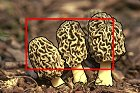
\includegraphics[height=1.75cm]{pictures/bsds500/gt/contours/marked/208078-1}\phantomsubcaption\label{subfig:datasets-bsds500}%
		\end{subfigure}
		\begin{subfigure}[t]{0.425\textwidth}%
			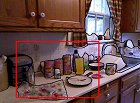
\includegraphics[height=1.75cm]{pictures/nyuv2/gt/contours/marked/00000561}\phantomsubcaption\label{subfig:datasets-nyuv2}%
		\end{subfigure}
		\\[4px]
		\begin{subfigure}[t]{0.5\textwidth}%
			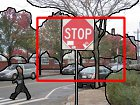
\includegraphics[height=1.75cm]{pictures/sbd/gt/contours/marked/6000067}\phantomsubcaption\label{subfig:datasets-sbd}%
		\end{subfigure}
		\begin{subfigure}[t]{0.425\textwidth}%
			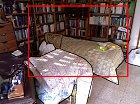
\includegraphics[height=1.75cm]{pictures/sunrgbd/gt/contours/marked/00007477}\phantomsubcaption\label{subfig:datasets-sunrgbd}%
		\end{subfigure}
	\end{subfigure}
	\hskip -3px
	\begin{subfigure}[t]{0.12\textwidth}%
		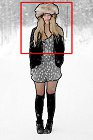
\includegraphics[height=3.68cm]{pictures/fash/gt/contours/marked/132}\phantomsubcaption\label{subfig:datasets-fash}%
	\end{subfigure}
	\caption{Example images from the used datasets. From left ro right: \BSDS; \SBD; \NYU; \SUNRGBD; and \Fash.
	Black contours represent ground truth and red rectangles indicate excerpts
	used for qualitative comparison in Figures \ref{fig:appendix-experiments-qualitative-bsds500-sbd-fash}
	and \ref{fig:appendix-experiments-qualitative-nyuv2-sunrgbd}.
	\textbf{Best viewed in color.}}
	\label{fig:appendix-datasets}
\end{figure}

The \BSDS dataset is the only dataset providing several ground truth segmentations per image.
Therefore, we briefly discuss evaluation on the \BSDS dataset in detail. Furthermore, 
additional example images from all used datasets are shown in Figure \ref{fig:appendix-datasets} and 
are used for qualitative results in \ref{subsec:appendix-experiments-qualitative}.

Assuming at least two ground truth segmentations per image, Arbel{\'a}ez \etal \cite{ArbelaezMaireFowlkesMalik:2011}
consider two methodologies of computing average \Rec: computing the average \Rec over all ground truth
segmentations per image, and subsequently taking the worst average (\ie the lowest \Rec); or taking the
lowest \Rec over all ground truth segmentations per image and averaging these. We follow Arbel{\'a}ez \etal
and pick the latter approach. The same methodology is then applied to \UE, \EV, \ASA and \UEL.
In this sense, we never overestimate performance with respect to the provided ground truth
segmentations.
